%%%%%%%%%%%%%%%%%%%%%%%INNLEDNING%%%%%%%%%%%%%%%%%%%%%%%%%%%%%%%%%%%%%%%%%%%%%%%%%%%%%%%%
%%%%%%This is normally Chapter 1 and gives an overview of the assignment and why this work is important. If you have chosen to focus mainly on a part of the assignment text, you may write something about this here and explain why. You also normally give a short description of the structure of the rest of the report towards the end of this chapter.  It is important to indicate which parts that are based on your own work. You may even include a list of your main contributions. %%%%%
\chapter{Introduction}
\pagenumbering{arabic}


%%%%%Introduksjon, GPS i IOT verden osv%%%%%%%

Internet of things (IoT) is the network which consists of objects that are connected to the internet such as sensors, vehicles, actuators and other embedded devices. The devices use the internet to deliver data or to be controlled remotely. IoT is used in the industry to improve the efficiency of operations, safety and security and give valuable insights in analyzing Big data. The use cases for IoT is also relevant for the general consumer as more of the objects in the household are connected to the Internet.For instance controlling the oven temperature with a mobile app or automatically notifying the hospital if an irregular heart rhythm is noticed by a person's pacemaker. IoT is one of the fastest growing trends in technology today, which is highlighted by Gartners Hype cycle of 2017 shown in figure \ref{fig:Gartner}


\begin{minipage}[H!]{0.8\textwidth}
    \centering
    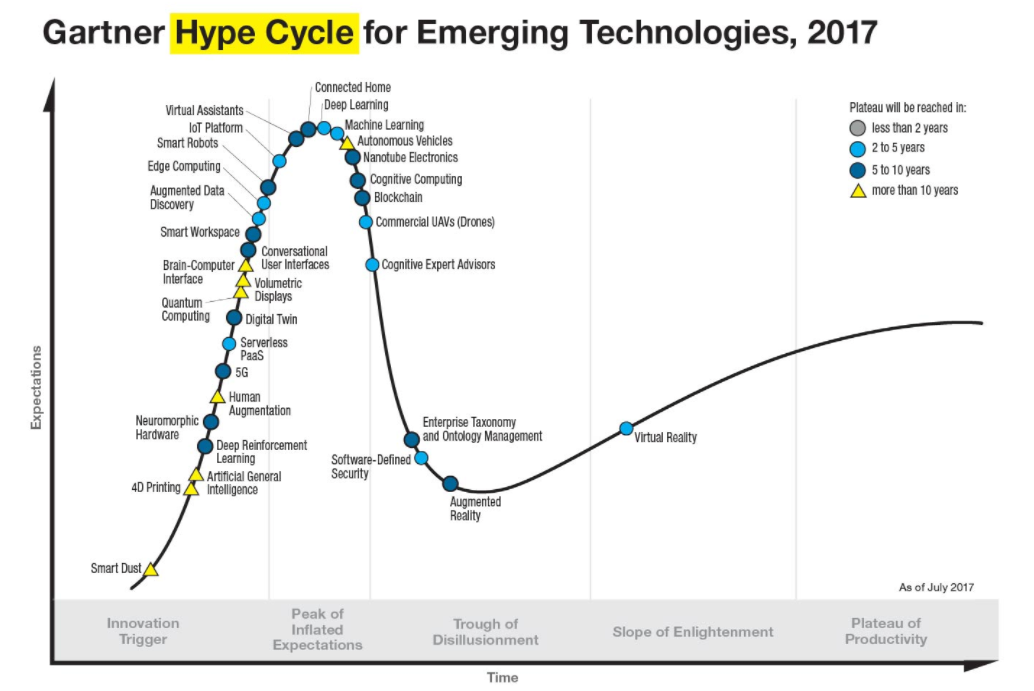
\includegraphics[width=1.2\textwidth]{Images/Gartner.PNG}\\
    \captionof{figure}{Gartners Hype Cycle 2017 with IoT as on of the fastest growing trends }
    \label{fig:Gartner}
\end{minipage}





In \cite{kraemer} Kraemer et al explains how most of the sensors that are deployed in the internet of things have high energy constraints and are dependent on using energy harvesting for sustaining their operation. Since many of the sensors are situated in heterogeneous environments that change over time, they are required to use an optimized energy consumption and harvesting technique to ensure a working state. But the internet of things is also characterized as a vast network of devices, which is predicted to grow from 4 billion devices to 20 billion in 2019 \cite{IEA}. Individually optimizing every sensor is therefore impractical. According to \cite{frank} these challenges can be summed up into tree key challenges: 
\begin{enumerate}
    \item The scale of connected devices in terms of units
    \item The constraints in terms of resources: energy, memory, computation
    \item The non-stationary and heterogeneous environments of things.
    \label{challenges}
    
\end{enumerate}

\subsection{Problem description}

As the  IoT continues to grow, other trends in technologies are becoming more developed. Cloud computing is one these trends  and enables the sensors to access unlimited of computation power\cite{Cloud}. Cloud storage enables the sensors to store the vast amount of big data that can be used to determine future behavior. While some of the challenges in \ref{challenges} can be overcome by using emerging technologies, the energy challenge in IoT is still not feasible to overcome. 

This project will attempt to solve some of the energy constraint IoT designers face today. The project shall explain and build a model of the energy consumption of an IoT device which uses the GPS. The model shall enable an application to determine the best energy strategy of getting a positional fix based on the energy model. 




\subsection{Motivation}

The project is part of a ongoing research project at the Faculty of Information Technology and Electronics at NTNU. The research project is called Autonomous Resource-Constrained Things(ART).  The ART project look at sensor devices as  smart robots that acts as autonomous agents, who have to plan ahead and make decisions instead of just sources of data \cite{kraemer}.The aim of the research project is to develop a method for AI to optimize the IoT infrastructure by using machine learning.

As part of the ART project Ameen Hussain has proposed and evaluated an energy consumption estimation approach for periodic sensing applications running on the IoT devices\cite{Amen}.As the position of an object is one of the most requested information for IoT applications, the usage of GPS has grown substantially.The GPS receiver is used in embedded systems such as watches, trackers, cellphones and cars. It is necessary to have an energy model of the GPS receiver, because it can be one of the most energy hungry devices in an IoT system. The combination of high energy demand and limited energy budget motivates the developing of an optimized energy strategy. 

The student's motivation for choosing this project was to have some insight and experience regarding the different technologies in IoT. The student thinks the experience will be beneficial later as IoT becomes a dominating trend in the Industry. Another motivation was that the Internet of Things combines multiple fields of technology, and challenges the student to apply all of his knowledge of IT and Electronics.


\subsection{Methodology}


The first step in optimizing the energy consumption was to understand the GPS system.Literature from  \cite{GPS} was mainly used for this purpose. The next step was to do a literary study of different methods for measuring the energy consumption, search engines that were used for this: Google Scholar and IEEE Xplorer. 
A decision of the measurement method was then done, based on the advantages and disadvantages which were highlighted by the literary study. Program code for the hardware and the experiment was then developed. Every component that was necessary for the measurements was mounted on a cycle wagon to make the measurement platform mobile. 

After the measurement platform was developed, we did measurements of the GPS system with different program code. Experiments was repeated up to 40 times. The data was compared with the knowledge that was acquired from the data sheet of the GPS and the knowledge from \cite{GPS} to confirm its validity. After we had acquired enough data, we did a parameter exploration for the energy model.The last step was to make an energy model based on the acquired knowledge and measurements of the GPS. 



\subsection{Report Structure}

WRITE THIS LATER 


\newpage